% Options for packages loaded elsewhere
\PassOptionsToPackage{unicode}{hyperref}
\PassOptionsToPackage{hyphens}{url}
\PassOptionsToPackage{dvipsnames,svgnames,x11names}{xcolor}
%
\documentclass[
  letterpaper,
  DIV=11,
  numbers=noendperiod]{scrartcl}

\usepackage{amsmath,amssymb}
\usepackage{lmodern}
\usepackage{iftex}
\ifPDFTeX
  \usepackage[T1]{fontenc}
  \usepackage[utf8]{inputenc}
  \usepackage{textcomp} % provide euro and other symbols
\else % if luatex or xetex
  \usepackage{unicode-math}
  \defaultfontfeatures{Scale=MatchLowercase}
  \defaultfontfeatures[\rmfamily]{Ligatures=TeX,Scale=1}
\fi
% Use upquote if available, for straight quotes in verbatim environments
\IfFileExists{upquote.sty}{\usepackage{upquote}}{}
\IfFileExists{microtype.sty}{% use microtype if available
  \usepackage[]{microtype}
  \UseMicrotypeSet[protrusion]{basicmath} % disable protrusion for tt fonts
}{}
\makeatletter
\@ifundefined{KOMAClassName}{% if non-KOMA class
  \IfFileExists{parskip.sty}{%
    \usepackage{parskip}
  }{% else
    \setlength{\parindent}{0pt}
    \setlength{\parskip}{6pt plus 2pt minus 1pt}}
}{% if KOMA class
  \KOMAoptions{parskip=half}}
\makeatother
\usepackage{xcolor}
\setlength{\emergencystretch}{3em} % prevent overfull lines
\setcounter{secnumdepth}{-\maxdimen} % remove section numbering
% Make \paragraph and \subparagraph free-standing
\ifx\paragraph\undefined\else
  \let\oldparagraph\paragraph
  \renewcommand{\paragraph}[1]{\oldparagraph{#1}\mbox{}}
\fi
\ifx\subparagraph\undefined\else
  \let\oldsubparagraph\subparagraph
  \renewcommand{\subparagraph}[1]{\oldsubparagraph{#1}\mbox{}}
\fi

\usepackage{color}
\usepackage{fancyvrb}
\newcommand{\VerbBar}{|}
\newcommand{\VERB}{\Verb[commandchars=\\\{\}]}
\DefineVerbatimEnvironment{Highlighting}{Verbatim}{commandchars=\\\{\}}
% Add ',fontsize=\small' for more characters per line
\usepackage{framed}
\definecolor{shadecolor}{RGB}{241,243,245}
\newenvironment{Shaded}{\begin{snugshade}}{\end{snugshade}}
\newcommand{\AlertTok}[1]{\textcolor[rgb]{0.68,0.00,0.00}{#1}}
\newcommand{\AnnotationTok}[1]{\textcolor[rgb]{0.37,0.37,0.37}{#1}}
\newcommand{\AttributeTok}[1]{\textcolor[rgb]{0.40,0.45,0.13}{#1}}
\newcommand{\BaseNTok}[1]{\textcolor[rgb]{0.68,0.00,0.00}{#1}}
\newcommand{\BuiltInTok}[1]{\textcolor[rgb]{0.00,0.23,0.31}{#1}}
\newcommand{\CharTok}[1]{\textcolor[rgb]{0.13,0.47,0.30}{#1}}
\newcommand{\CommentTok}[1]{\textcolor[rgb]{0.37,0.37,0.37}{#1}}
\newcommand{\CommentVarTok}[1]{\textcolor[rgb]{0.37,0.37,0.37}{\textit{#1}}}
\newcommand{\ConstantTok}[1]{\textcolor[rgb]{0.56,0.35,0.01}{#1}}
\newcommand{\ControlFlowTok}[1]{\textcolor[rgb]{0.00,0.23,0.31}{#1}}
\newcommand{\DataTypeTok}[1]{\textcolor[rgb]{0.68,0.00,0.00}{#1}}
\newcommand{\DecValTok}[1]{\textcolor[rgb]{0.68,0.00,0.00}{#1}}
\newcommand{\DocumentationTok}[1]{\textcolor[rgb]{0.37,0.37,0.37}{\textit{#1}}}
\newcommand{\ErrorTok}[1]{\textcolor[rgb]{0.68,0.00,0.00}{#1}}
\newcommand{\ExtensionTok}[1]{\textcolor[rgb]{0.00,0.23,0.31}{#1}}
\newcommand{\FloatTok}[1]{\textcolor[rgb]{0.68,0.00,0.00}{#1}}
\newcommand{\FunctionTok}[1]{\textcolor[rgb]{0.28,0.35,0.67}{#1}}
\newcommand{\ImportTok}[1]{\textcolor[rgb]{0.00,0.46,0.62}{#1}}
\newcommand{\InformationTok}[1]{\textcolor[rgb]{0.37,0.37,0.37}{#1}}
\newcommand{\KeywordTok}[1]{\textcolor[rgb]{0.00,0.23,0.31}{#1}}
\newcommand{\NormalTok}[1]{\textcolor[rgb]{0.00,0.23,0.31}{#1}}
\newcommand{\OperatorTok}[1]{\textcolor[rgb]{0.37,0.37,0.37}{#1}}
\newcommand{\OtherTok}[1]{\textcolor[rgb]{0.00,0.23,0.31}{#1}}
\newcommand{\PreprocessorTok}[1]{\textcolor[rgb]{0.68,0.00,0.00}{#1}}
\newcommand{\RegionMarkerTok}[1]{\textcolor[rgb]{0.00,0.23,0.31}{#1}}
\newcommand{\SpecialCharTok}[1]{\textcolor[rgb]{0.37,0.37,0.37}{#1}}
\newcommand{\SpecialStringTok}[1]{\textcolor[rgb]{0.13,0.47,0.30}{#1}}
\newcommand{\StringTok}[1]{\textcolor[rgb]{0.13,0.47,0.30}{#1}}
\newcommand{\VariableTok}[1]{\textcolor[rgb]{0.07,0.07,0.07}{#1}}
\newcommand{\VerbatimStringTok}[1]{\textcolor[rgb]{0.13,0.47,0.30}{#1}}
\newcommand{\WarningTok}[1]{\textcolor[rgb]{0.37,0.37,0.37}{\textit{#1}}}

\providecommand{\tightlist}{%
  \setlength{\itemsep}{0pt}\setlength{\parskip}{0pt}}\usepackage{longtable,booktabs,array}
\usepackage{calc} % for calculating minipage widths
% Correct order of tables after \paragraph or \subparagraph
\usepackage{etoolbox}
\makeatletter
\patchcmd\longtable{\par}{\if@noskipsec\mbox{}\fi\par}{}{}
\makeatother
% Allow footnotes in longtable head/foot
\IfFileExists{footnotehyper.sty}{\usepackage{footnotehyper}}{\usepackage{footnote}}
\makesavenoteenv{longtable}
\usepackage{graphicx}
\makeatletter
\def\maxwidth{\ifdim\Gin@nat@width>\linewidth\linewidth\else\Gin@nat@width\fi}
\def\maxheight{\ifdim\Gin@nat@height>\textheight\textheight\else\Gin@nat@height\fi}
\makeatother
% Scale images if necessary, so that they will not overflow the page
% margins by default, and it is still possible to overwrite the defaults
% using explicit options in \includegraphics[width, height, ...]{}
\setkeys{Gin}{width=\maxwidth,height=\maxheight,keepaspectratio}
% Set default figure placement to htbp
\makeatletter
\def\fps@figure{htbp}
\makeatother

\usepackage{booktabs}
\usepackage{longtable}
\usepackage{array}
\usepackage{multirow}
\usepackage{wrapfig}
\usepackage{float}
\usepackage{colortbl}
\usepackage{pdflscape}
\usepackage{tabu}
\usepackage{threeparttable}
\usepackage{threeparttablex}
\usepackage[normalem]{ulem}
\usepackage{makecell}
\usepackage{xcolor}
\KOMAoption{captions}{tableheading}
\makeatletter
\makeatother
\makeatletter
\makeatother
\makeatletter
\@ifpackageloaded{caption}{}{\usepackage{caption}}
\AtBeginDocument{%
\ifdefined\contentsname
  \renewcommand*\contentsname{Table of contents}
\else
  \newcommand\contentsname{Table of contents}
\fi
\ifdefined\listfigurename
  \renewcommand*\listfigurename{List of Figures}
\else
  \newcommand\listfigurename{List of Figures}
\fi
\ifdefined\listtablename
  \renewcommand*\listtablename{List of Tables}
\else
  \newcommand\listtablename{List of Tables}
\fi
\ifdefined\figurename
  \renewcommand*\figurename{Figure}
\else
  \newcommand\figurename{Figure}
\fi
\ifdefined\tablename
  \renewcommand*\tablename{Table}
\else
  \newcommand\tablename{Table}
\fi
}
\@ifpackageloaded{float}{}{\usepackage{float}}
\floatstyle{ruled}
\@ifundefined{c@chapter}{\newfloat{codelisting}{h}{lop}}{\newfloat{codelisting}{h}{lop}[chapter]}
\floatname{codelisting}{Listing}
\newcommand*\listoflistings{\listof{codelisting}{List of Listings}}
\makeatother
\makeatletter
\@ifpackageloaded{caption}{}{\usepackage{caption}}
\@ifpackageloaded{subcaption}{}{\usepackage{subcaption}}
\makeatother
\makeatletter
\@ifpackageloaded{tcolorbox}{}{\usepackage[many]{tcolorbox}}
\makeatother
\makeatletter
\@ifundefined{shadecolor}{\definecolor{shadecolor}{rgb}{.97, .97, .97}}
\makeatother
\makeatletter
\makeatother
\ifLuaTeX
  \usepackage{selnolig}  % disable illegal ligatures
\fi
\IfFileExists{bookmark.sty}{\usepackage{bookmark}}{\usepackage{hyperref}}
\IfFileExists{xurl.sty}{\usepackage{xurl}}{} % add URL line breaks if available
\urlstyle{same} % disable monospaced font for URLs
\hypersetup{
  pdftitle={Cement Productioin in Pakistan},
  pdfauthor={Zahid Asghar},
  colorlinks=true,
  linkcolor={blue},
  filecolor={Maroon},
  citecolor={Blue},
  urlcolor={Blue},
  pdfcreator={LaTeX via pandoc}}

\title{Cement Productioin in Pakistan}
\author{\emph{Zahid Asghar}}
\date{10 October 2022}

\begin{document}
\maketitle
\ifdefined\Shaded\renewenvironment{Shaded}{\begin{tcolorbox}[enhanced, sharp corners, frame hidden, borderline west={3pt}{0pt}{shadecolor}, interior hidden, breakable, boxrule=0pt]}{\end{tcolorbox}}\fi

\hypertarget{section}{%
\subsection{\texorpdfstring{\protect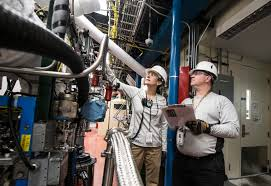
\includegraphics[width=16.66667in,height=8.33333in]{industry.jpg}}{}}\label{section}}

\hypertarget{cement-production}{%
\subsection{Cement Production}\label{cement-production}}

We have data from \href{https://www.apcma.com}{Cement Manufacturers
Association}. Lets explore this data as follows:

\begin{Shaded}
\begin{Highlighting}[]
\FunctionTok{library}\NormalTok{(tidyverse)}
\FunctionTok{library}\NormalTok{(lubridate)}
\FunctionTok{library}\NormalTok{(readr)}
\FunctionTok{library}\NormalTok{(readxl)}
\FunctionTok{library}\NormalTok{(collapse)}
\FunctionTok{library}\NormalTok{(kableExtra)}
\FunctionTok{library}\NormalTok{(dynlm)}
\FunctionTok{library}\NormalTok{(forecast)}
\FunctionTok{library}\NormalTok{(stargazer)}
\FunctionTok{library}\NormalTok{(scales)}
\FunctionTok{library}\NormalTok{(xts)}
\FunctionTok{library}\NormalTok{(urca)}
\FunctionTok{library}\NormalTok{(tsibble)}
\FunctionTok{library}\NormalTok{(fpp2)}
\FunctionTok{library}\NormalTok{(fpp3)}
\FunctionTok{library}\NormalTok{(ggthemes)}
\FunctionTok{library}\NormalTok{(DT)}
\FunctionTok{library}\NormalTok{(fable)}
\FunctionTok{library}\NormalTok{(fabletools)}
\end{Highlighting}
\end{Shaded}

\hypertarget{read-data}{%
\subsubsection{Read data}\label{read-data}}

\begin{Shaded}
\begin{Highlighting}[]
\FunctionTok{library}\NormalTok{(readr) }\CommentTok{\# To load data from csv file, if one needs to load data from excel, then use excel file}
\NormalTok{cement}\OtherTok{\textless{}{-}}\FunctionTok{read\_csv}\NormalTok{(}\StringTok{"cement.csv"}\NormalTok{)}
\FunctionTok{glimpse}\NormalTok{(cement)}
\DocumentationTok{\#\# Rows: 1,116}
\DocumentationTok{\#\# Columns: 6}
\DocumentationTok{\#\# $ Date                         \textless{}chr\textgreater{} "07/1991", "07/1991", "07/1991", "08\textasciitilde{}}
\DocumentationTok{\#\# $ \textasciigrave{}Series Name\textasciigrave{}                \textless{}chr\textgreater{} "Total Cement Sales", "Domestic Ceme\textasciitilde{}}
\DocumentationTok{\#\# $ Output                       \textless{}dbl\textgreater{} 599, 599, NA, 632, 632, NA, 633, 633\textasciitilde{}}
\DocumentationTok{\#\# $ Unit                         \textless{}chr\textgreater{} "Thousand Metric Ton", "Thousand Met\textasciitilde{}}
\DocumentationTok{\#\# $ \textasciigrave{}Observation Status\textasciigrave{}         \textless{}chr\textgreater{} "Normal", "Normal", "Missing value",\textasciitilde{}}
\DocumentationTok{\#\# $ \textasciigrave{}Observation Status Comment\textasciigrave{} \textless{}lgl\textgreater{} NA, NA, NA, NA, NA, NA, NA, NA, NA, \textasciitilde{}}
\end{Highlighting}
\end{Shaded}

\hypertarget{selecting-and-renaming-variables}{%
\subsubsection{Selecting and Renaming
variables}\label{selecting-and-renaming-variables}}

\begin{Shaded}
\begin{Highlighting}[]
\NormalTok{cement}\OtherTok{\textless{}{-}}\NormalTok{cement }\SpecialCharTok{\%\textgreater{}\%} \FunctionTok{rename}\NormalTok{(}\AttributeTok{Category=}\StringTok{\textasciigrave{}}\AttributeTok{Series Name}\StringTok{\textasciigrave{}}\NormalTok{ )}

\CommentTok{\#cement\textless{}{-}ts(cement, frequency = 12, start=c(1991,7))}
\CommentTok{\#cement}
\CommentTok{\#cement\textless{}{-}cement \%\textgreater{}\% mutate(Month=yearmonth(Date)) \%\textgreater{}\% as\_tsibble(index = Month)}

\NormalTok{cement}\OtherTok{\textless{}{-}}\NormalTok{cement }\SpecialCharTok{\%\textgreater{}\%} \FunctionTok{filter}\NormalTok{(Category}\SpecialCharTok{==}\StringTok{"Total Cement Sales"}\NormalTok{) }\CommentTok{\# Select only Total Cement Sales}

\NormalTok{cement}\SpecialCharTok{$}\NormalTok{Date}\OtherTok{\textless{}{-}}\FunctionTok{my}\NormalTok{(cement}\SpecialCharTok{$}\NormalTok{Date) }\CommentTok{\# Formating required}
\NormalTok{cement}\SpecialCharTok{$}\NormalTok{Date}\OtherTok{\textless{}{-}}\FunctionTok{as\_date}\NormalTok{(cement}\SpecialCharTok{$}\NormalTok{Date,}\AttributeTok{format=}\StringTok{"\%Y{-}\%m"}\NormalTok{)}

\CommentTok{\#cement\textless{}{-}tsibble(cement)}
\NormalTok{cement}
\DocumentationTok{\#\# \# A tibble: 372 x 6}
\DocumentationTok{\#\#    Date       Category           Output Unit                Obser\textasciitilde{}1 Obser\textasciitilde{}2}
\DocumentationTok{\#\#    \textless{}date\textgreater{}     \textless{}chr\textgreater{}               \textless{}dbl\textgreater{} \textless{}chr\textgreater{}               \textless{}chr\textgreater{}   \textless{}lgl\textgreater{}  }
\DocumentationTok{\#\#  1 1991{-}07{-}01 Total Cement Sales   599. Thousand Metric Ton Normal  NA     }
\DocumentationTok{\#\#  2 1991{-}08{-}01 Total Cement Sales   632. Thousand Metric Ton Normal  NA     }
\DocumentationTok{\#\#  3 1991{-}09{-}01 Total Cement Sales   633  Thousand Metric Ton Normal  NA     }
\DocumentationTok{\#\#  4 1991{-}10{-}01 Total Cement Sales   701. Thousand Metric Ton Normal  NA     }
\DocumentationTok{\#\#  5 1991{-}11{-}01 Total Cement Sales   635. Thousand Metric Ton Normal  NA     }
\DocumentationTok{\#\#  6 1991{-}12{-}01 Total Cement Sales   689. Thousand Metric Ton Normal  NA     }
\DocumentationTok{\#\#  7 1992{-}01{-}01 Total Cement Sales   580. Thousand Metric Ton Normal  NA     }
\DocumentationTok{\#\#  8 1992{-}02{-}01 Total Cement Sales   612. Thousand Metric Ton Normal  NA     }
\DocumentationTok{\#\#  9 1992{-}03{-}01 Total Cement Sales   725. Thousand Metric Ton Normal  NA     }
\DocumentationTok{\#\# 10 1992{-}04{-}01 Total Cement Sales   641. Thousand Metric Ton Normal  NA     }
\DocumentationTok{\#\# \# ... with 362 more rows, and abbreviated variable names}
\DocumentationTok{\#\# \#   1: \textasciigrave{}Observation Status\textasciigrave{}, 2: \textasciigrave{}Observation Status Comment\textasciigrave{}}
\DocumentationTok{\#\# \# i Use \textasciigrave{}print(n = ...)\textasciigrave{} to see more rows}
\NormalTok{cement}\SpecialCharTok{$}\NormalTok{year}\OtherTok{\textless{}{-}}\FunctionTok{year}\NormalTok{(cement}\SpecialCharTok{$}\NormalTok{Date)}
\NormalTok{cement}
\DocumentationTok{\#\# \# A tibble: 372 x 7}
\DocumentationTok{\#\#    Date       Category           Output Unit          Obser\textasciitilde{}1 Obser\textasciitilde{}2  year}
\DocumentationTok{\#\#    \textless{}date\textgreater{}     \textless{}chr\textgreater{}               \textless{}dbl\textgreater{} \textless{}chr\textgreater{}         \textless{}chr\textgreater{}   \textless{}lgl\textgreater{}   \textless{}dbl\textgreater{}}
\DocumentationTok{\#\#  1 1991{-}07{-}01 Total Cement Sales   599. Thousand Met\textasciitilde{} Normal  NA       1991}
\DocumentationTok{\#\#  2 1991{-}08{-}01 Total Cement Sales   632. Thousand Met\textasciitilde{} Normal  NA       1991}
\DocumentationTok{\#\#  3 1991{-}09{-}01 Total Cement Sales   633  Thousand Met\textasciitilde{} Normal  NA       1991}
\DocumentationTok{\#\#  4 1991{-}10{-}01 Total Cement Sales   701. Thousand Met\textasciitilde{} Normal  NA       1991}
\DocumentationTok{\#\#  5 1991{-}11{-}01 Total Cement Sales   635. Thousand Met\textasciitilde{} Normal  NA       1991}
\DocumentationTok{\#\#  6 1991{-}12{-}01 Total Cement Sales   689. Thousand Met\textasciitilde{} Normal  NA       1991}
\DocumentationTok{\#\#  7 1992{-}01{-}01 Total Cement Sales   580. Thousand Met\textasciitilde{} Normal  NA       1992}
\DocumentationTok{\#\#  8 1992{-}02{-}01 Total Cement Sales   612. Thousand Met\textasciitilde{} Normal  NA       1992}
\DocumentationTok{\#\#  9 1992{-}03{-}01 Total Cement Sales   725. Thousand Met\textasciitilde{} Normal  NA       1992}
\DocumentationTok{\#\# 10 1992{-}04{-}01 Total Cement Sales   641. Thousand Met\textasciitilde{} Normal  NA       1992}
\DocumentationTok{\#\# \# ... with 362 more rows, and abbreviated variable names}
\DocumentationTok{\#\# \#   1: \textasciigrave{}Observation Status\textasciigrave{}, 2: \textasciigrave{}Observation Status Comment\textasciigrave{}}
\DocumentationTok{\#\# \# i Use \textasciigrave{}print(n = ...)\textasciigrave{} to see more rows}
\NormalTok{cement\_yrly}\OtherTok{\textless{}{-}}\NormalTok{cement }\SpecialCharTok{\%\textgreater{}\%} \FunctionTok{group\_by}\NormalTok{(year) }\SpecialCharTok{\%\textgreater{}\%} \FunctionTok{summarise}\NormalTok{(}\AttributeTok{prod\_yr=}\FunctionTok{sum}\NormalTok{(Output))}
\NormalTok{cement\_yrly}\OtherTok{\textless{}{-}}\NormalTok{cement\_yrly }\SpecialCharTok{\%\textgreater{}\%} \FunctionTok{filter}\NormalTok{(year}\SpecialCharTok{\textless{}=}\DecValTok{2021}\NormalTok{)}
\CommentTok{\#cement\_yrly$year\textless{}{-}make\_date(cement\_yrly$year)}
\CommentTok{\#cement\_yrly\textless{}{-}tsibble(cement\_yrly)}
\NormalTok{cement\_yrly}
\DocumentationTok{\#\# \# A tibble: 31 x 2}
\DocumentationTok{\#\#     year prod\_yr}
\DocumentationTok{\#\#    \textless{}dbl\textgreater{}   \textless{}dbl\textgreater{}}
\DocumentationTok{\#\#  1  1991   3890.}
\DocumentationTok{\#\#  2  1992   7504.}
\DocumentationTok{\#\#  3  1993   8092.}
\DocumentationTok{\#\#  4  1994   7746.}
\DocumentationTok{\#\#  5  1995   8992.}
\DocumentationTok{\#\#  6  1996   9658.}
\DocumentationTok{\#\#  7  1997   9519.}
\DocumentationTok{\#\#  8  1998   9324.}
\DocumentationTok{\#\#  9  1999   9585 }
\DocumentationTok{\#\# 10  2000   9882.}
\DocumentationTok{\#\# \# ... with 21 more rows}
\DocumentationTok{\#\# \# i Use \textasciigrave{}print(n = ...)\textasciigrave{} to see more rows}
\CommentTok{\#cement\textless{}{-}tsibble(cement)}
\end{Highlighting}
\end{Shaded}

\hypertarget{annual-cement-sale}{%
\subsection{Annual cement sale}\label{annual-cement-sale}}

\hypertarget{what-happens-if-year-2022-is-included}{%
\subsubsection{What happens if year 2022 is
included?}\label{what-happens-if-year-2022-is-included}}

\hypertarget{why-annual-is-less-informative}{%
\subsubsection{Why annual is less
informative?}\label{why-annual-is-less-informative}}

\begin{Shaded}
\begin{Highlighting}[]
\NormalTok{p1}\OtherTok{\textless{}{-}}\FunctionTok{ggplot}\NormalTok{(cement\_yrly)}\SpecialCharTok{+}\FunctionTok{aes}\NormalTok{(}\AttributeTok{x=}\NormalTok{year,}\AttributeTok{y=}\NormalTok{prod\_yr)}\SpecialCharTok{+}\FunctionTok{geom\_line}\NormalTok{()}
\NormalTok{p1}
\end{Highlighting}
\end{Shaded}

\begin{figure}[H]

{\centering 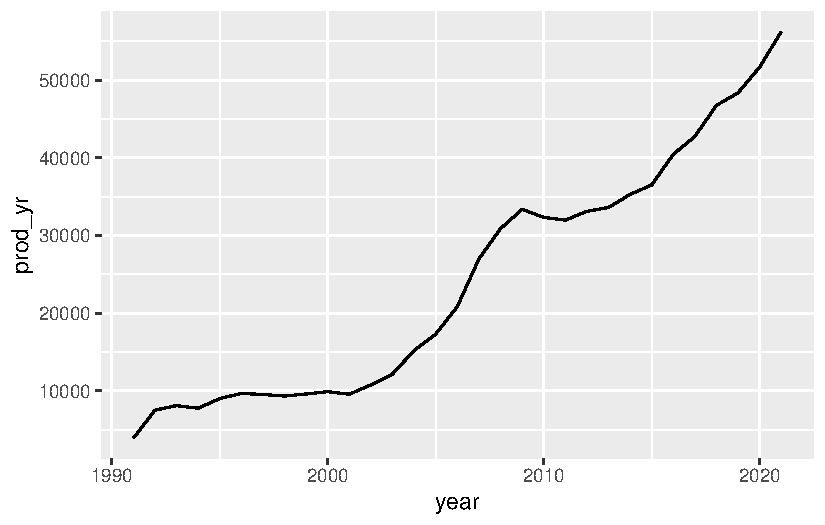
\includegraphics[width=17.1875in,height=\textheight]{cement_files/figure-pdf/unnamed-chunk-5-1.pdf}

}

\end{figure}

\begin{Shaded}
\begin{Highlighting}[]
\NormalTok{forecast}\SpecialCharTok{::}\FunctionTok{naive}\NormalTok{(cement\_yrly}\SpecialCharTok{$}\NormalTok{prod\_yr, }\AttributeTok{h=}\DecValTok{4}\NormalTok{) }\SpecialCharTok{\%\textgreater{}\%} \FunctionTok{autoplot}\NormalTok{() }
\end{Highlighting}
\end{Shaded}

\begin{figure}[H]

{\centering 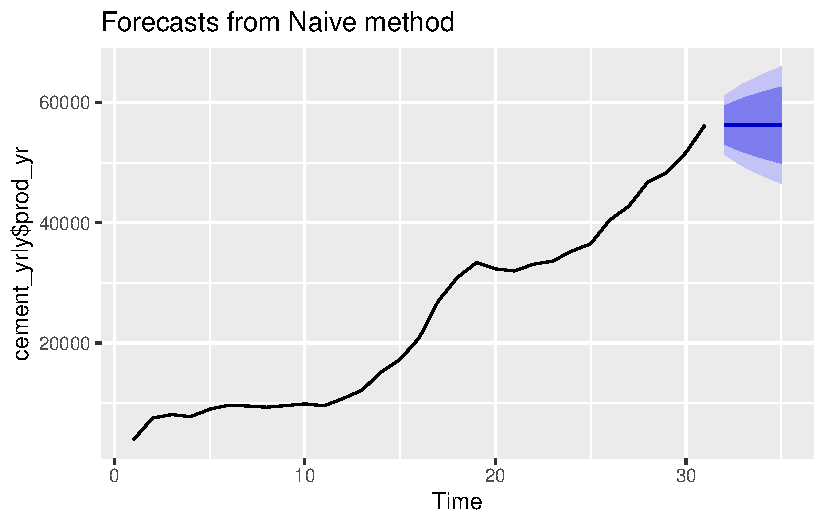
\includegraphics[width=17.1875in,height=\textheight]{cement_files/figure-pdf/unnamed-chunk-5-2.pdf}

}

\end{figure}

\hypertarget{monthly-cement-production}{%
\subsection{Monthly cement production}\label{monthly-cement-production}}

\begin{Shaded}
\begin{Highlighting}[]
\NormalTok{pm}\OtherTok{\textless{}{-}}\FunctionTok{ggplot}\NormalTok{(cement)}\SpecialCharTok{+}\FunctionTok{aes}\NormalTok{(}\AttributeTok{x=}\NormalTok{Date,}\AttributeTok{y=}\NormalTok{Output)}\SpecialCharTok{+}\FunctionTok{geom\_line}\NormalTok{()}
\NormalTok{pm}
\end{Highlighting}
\end{Shaded}

\begin{figure}[H]

{\centering 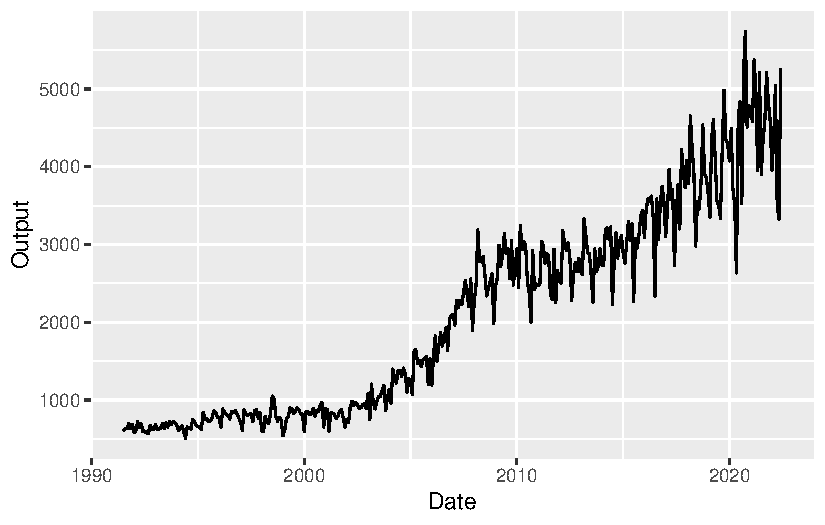
\includegraphics[width=17.1875in,height=\textheight]{cement_files/figure-pdf/unnamed-chunk-6-1.pdf}

}

\end{figure}

\hypertarget{labels-data-source-theme}{%
\subsection{Labels, data source, theme}\label{labels-data-source-theme}}

\begin{Shaded}
\begin{Highlighting}[]
\NormalTok{p1}\SpecialCharTok{+}\FunctionTok{labs}\NormalTok{(}\AttributeTok{x=}\StringTok{"Date"}\NormalTok{,}\AttributeTok{y=}\StringTok{"output (Thousand metric tons)"}\NormalTok{, }\AttributeTok{title =} \StringTok{"Year Production from 1991{-}2022"}\NormalTok{, }\AttributeTok{caption =} \StringTok{"By Zahid Asghar, Source:APCMA, Pakistan"}\NormalTok{)}
\end{Highlighting}
\end{Shaded}

\begin{figure}[H]

{\centering 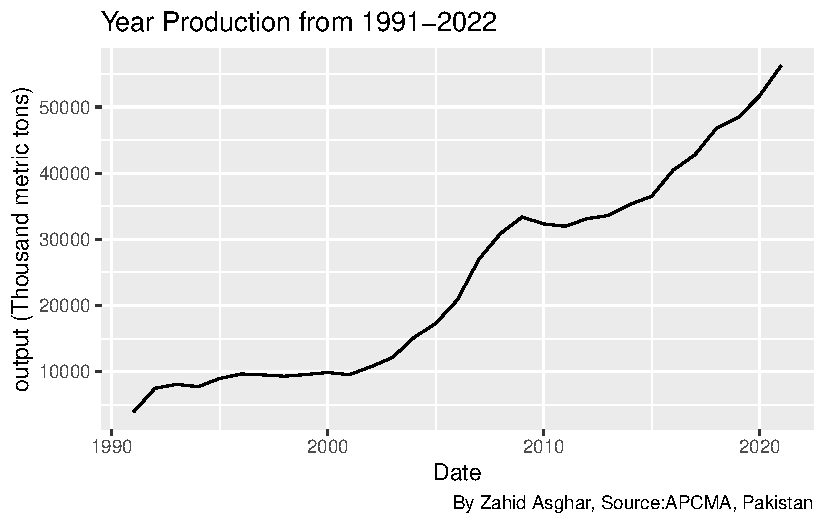
\includegraphics[width=17.1875in,height=\textheight]{cement_files/figure-pdf/unnamed-chunk-7-1.pdf}

}

\end{figure}

\hypertarget{section-1}{%
\subsection{}\label{section-1}}

\begin{Shaded}
\begin{Highlighting}[]
\NormalTok{pm}\SpecialCharTok{+}\FunctionTok{labs}\NormalTok{(}\AttributeTok{x=}\StringTok{"Date"}\NormalTok{,}\AttributeTok{y=}\StringTok{"Production (Thousand metric tons)"}\NormalTok{, }\AttributeTok{title =} \StringTok{"Year Production from 1991{-}2022"}\NormalTok{, }\AttributeTok{caption =} \StringTok{"By Zahid Asghar, Source:APCMA, Pakistan"}\NormalTok{)}
\end{Highlighting}
\end{Shaded}

\begin{figure}[H]

{\centering 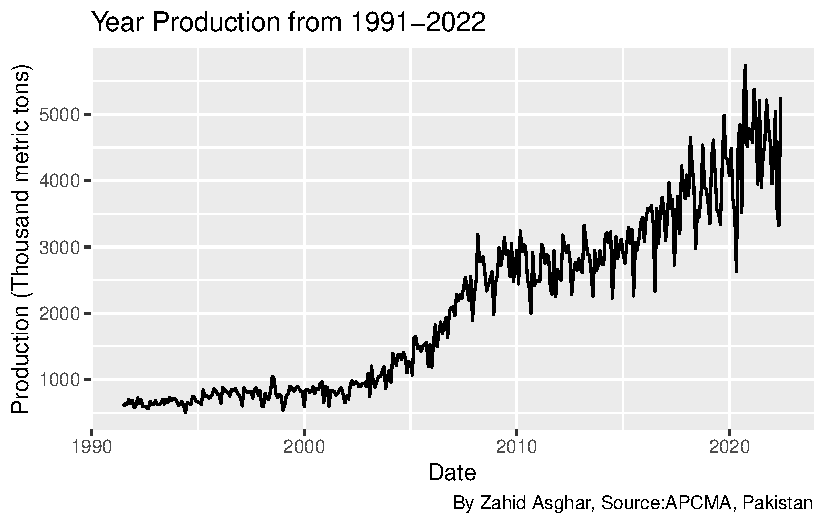
\includegraphics[width=17.1875in,height=\textheight]{cement_files/figure-pdf/unnamed-chunk-8-1.pdf}

}

\end{figure}

\hypertarget{last-10-years-data}{%
\subsection{Last 10 years data}\label{last-10-years-data}}

\begin{Shaded}
\begin{Highlighting}[]
\NormalTok{cement\_2010}\OtherTok{\textless{}{-}}\NormalTok{cement }\SpecialCharTok{\%\textgreater{}\%} \FunctionTok{filter}\NormalTok{(Date}\SpecialCharTok{\textgreater{}=}\StringTok{"2010{-}6{-}30"}\NormalTok{)}
\NormalTok{cement\_2010}
\DocumentationTok{\#\# \# A tibble: 144 x 7}
\DocumentationTok{\#\#    Date       Category           Output Unit          Obser\textasciitilde{}1 Obser\textasciitilde{}2  year}
\DocumentationTok{\#\#    \textless{}date\textgreater{}     \textless{}chr\textgreater{}               \textless{}dbl\textgreater{} \textless{}chr\textgreater{}         \textless{}chr\textgreater{}   \textless{}lgl\textgreater{}   \textless{}dbl\textgreater{}}
\DocumentationTok{\#\#  1 2010{-}07{-}01 Total Cement Sales  2524. Thousand Met\textasciitilde{} Normal  NA       2010}
\DocumentationTok{\#\#  2 2010{-}08{-}01 Total Cement Sales  2383. Thousand Met\textasciitilde{} Normal  NA       2010}
\DocumentationTok{\#\#  3 2010{-}09{-}01 Total Cement Sales  2002. Thousand Met\textasciitilde{} Normal  NA       2010}
\DocumentationTok{\#\#  4 2010{-}10{-}01 Total Cement Sales  2920. Thousand Met\textasciitilde{} Normal  NA       2010}
\DocumentationTok{\#\#  5 2010{-}11{-}01 Total Cement Sales  2416. Thousand Met\textasciitilde{} Normal  NA       2010}
\DocumentationTok{\#\#  6 2010{-}12{-}01 Total Cement Sales  2493. Thousand Met\textasciitilde{} Normal  NA       2010}
\DocumentationTok{\#\#  7 2011{-}01{-}01 Total Cement Sales  2473. Thousand Met\textasciitilde{} Normal  NA       2011}
\DocumentationTok{\#\#  8 2011{-}02{-}01 Total Cement Sales  2488. Thousand Met\textasciitilde{} Normal  NA       2011}
\DocumentationTok{\#\#  9 2011{-}03{-}01 Total Cement Sales  3043. Thousand Met\textasciitilde{} Normal  NA       2011}
\DocumentationTok{\#\# 10 2011{-}04{-}01 Total Cement Sales  2980. Thousand Met\textasciitilde{} Normal  NA       2011}
\DocumentationTok{\#\# \# ... with 134 more rows, and abbreviated variable names}
\DocumentationTok{\#\# \#   1: \textasciigrave{}Observation Status\textasciigrave{}, 2: \textasciigrave{}Observation Status Comment\textasciigrave{}}
\DocumentationTok{\#\# \# i Use \textasciigrave{}print(n = ...)\textasciigrave{} to see more rows}
\end{Highlighting}
\end{Shaded}

\begin{Shaded}
\begin{Highlighting}[]
\NormalTok{p11}\OtherTok{\textless{}{-}}\FunctionTok{ggplot}\NormalTok{(cement\_2010)}\SpecialCharTok{+}\FunctionTok{aes}\NormalTok{(}\AttributeTok{x=}\NormalTok{Date,}\AttributeTok{y=}\NormalTok{Output)}\SpecialCharTok{+}\FunctionTok{geom\_line}\NormalTok{()}
\NormalTok{p11}\SpecialCharTok{+}\FunctionTok{labs}\NormalTok{(}\AttributeTok{x=}\StringTok{"Date"}\NormalTok{,}\AttributeTok{y=}\StringTok{"Output (Thousand metric tons"}\NormalTok{, }\AttributeTok{title =} \StringTok{"Monthly Cement Output from 2010{-}2022"}\NormalTok{, }\AttributeTok{caption =} \StringTok{"By Zahid Asghar, Source:APCMA, Pakistan"}\NormalTok{)}
\end{Highlighting}
\end{Shaded}

\begin{figure}[H]

{\centering 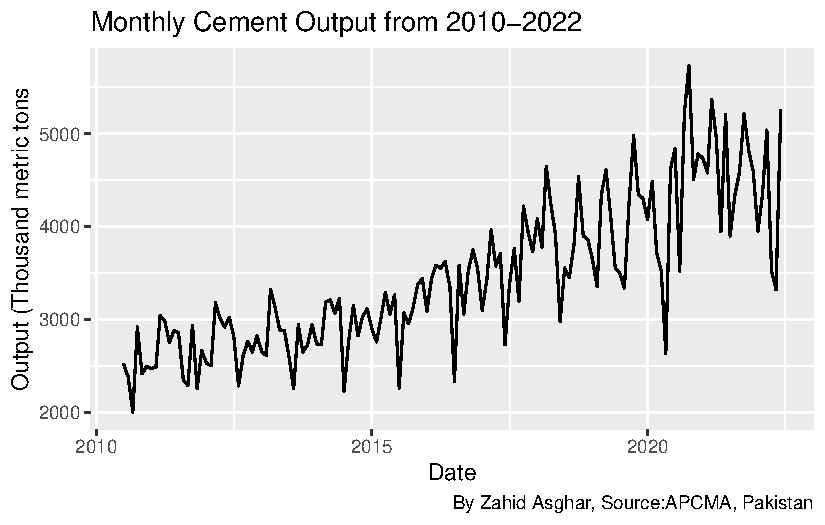
\includegraphics[width=17.1875in,height=\textheight]{cement_files/figure-pdf/unnamed-chunk-10-1.pdf}

}

\end{figure}

\hypertarget{forecasting}{%
\subsection{Forecasting}\label{forecasting}}

Why series seems reversed? This is because date is placed in reverse
order. So lets use a verb for sorting date in ascending order by
\texttt{sort}

\begin{Shaded}
\begin{Highlighting}[]

\NormalTok{forecast}\SpecialCharTok{::}\FunctionTok{snaive}\NormalTok{((cement}\SpecialCharTok{$}\NormalTok{Output), }\AttributeTok{h =} \DecValTok{24}\NormalTok{) }\SpecialCharTok{\%\textgreater{}\%} \FunctionTok{autoplot}\NormalTok{()}
\end{Highlighting}
\end{Shaded}

\begin{figure}[H]

{\centering 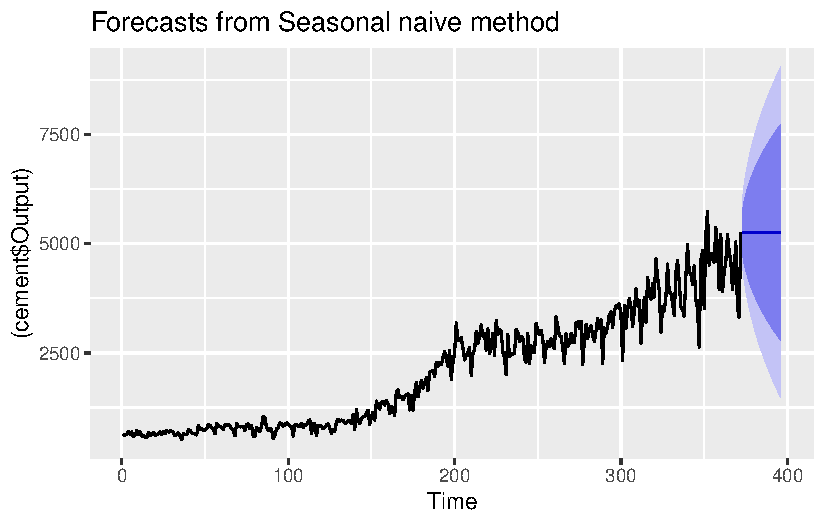
\includegraphics[width=17.1875in,height=\textheight]{cement_files/figure-pdf/unnamed-chunk-11-1.pdf}

}

\end{figure}

\hypertarget{arima-models}{%
\subsection{ARIMA models}\label{arima-models}}

\begin{verbatim}
## Series: cement$Output 
## ARIMA(4,1,1) with drift 
## 
## Coefficients:
##         ar1     ar2    ar3     ar4    ma1  drift
##       0.137  -0.106  0.082  -0.169  -0.83  10.54
## s.e.  0.064   0.059  0.059   0.057   0.04   2.67
## 
## sigma^2 = 100902:  log likelihood = -2661
## AIC=5337   AICc=5337   BIC=5364
## 
## Training set error measures:
##                  ME RMSE MAE   MPE MAPE  MASE     ACF1
## Training set -0.403  315 202 -2.99 10.1 0.811 -0.00574
\end{verbatim}

\hypertarget{seasonal-plot}{%
\subsection{Seasonal Plot}\label{seasonal-plot}}

\begin{Shaded}
\begin{Highlighting}[]
\NormalTok{cement}\OtherTok{\textless{}{-}}\NormalTok{cement }\SpecialCharTok{\%\textgreater{}\%} \FunctionTok{mutate}\NormalTok{(}\AttributeTok{Month=}\FunctionTok{yearmonth}\NormalTok{(Date)) }\SpecialCharTok{\%\textgreater{}\%} \FunctionTok{as\_tsibble}\NormalTok{(}\AttributeTok{index=}\NormalTok{Month)}

\NormalTok{cement }\SpecialCharTok{\%\textgreater{}\%}
  \FunctionTok{gg\_season}\NormalTok{(Output,}\AttributeTok{labels =} \StringTok{"both"}\NormalTok{)}\SpecialCharTok{+}
  \FunctionTok{labs}\NormalTok{(}\AttributeTok{y =} \StringTok{"$ (millions)"}\NormalTok{,}
       \AttributeTok{title =} \StringTok{"Seasonal plot: Antidiabetic drug sales"}\NormalTok{)}
\end{Highlighting}
\end{Shaded}

\begin{figure}[H]

{\centering 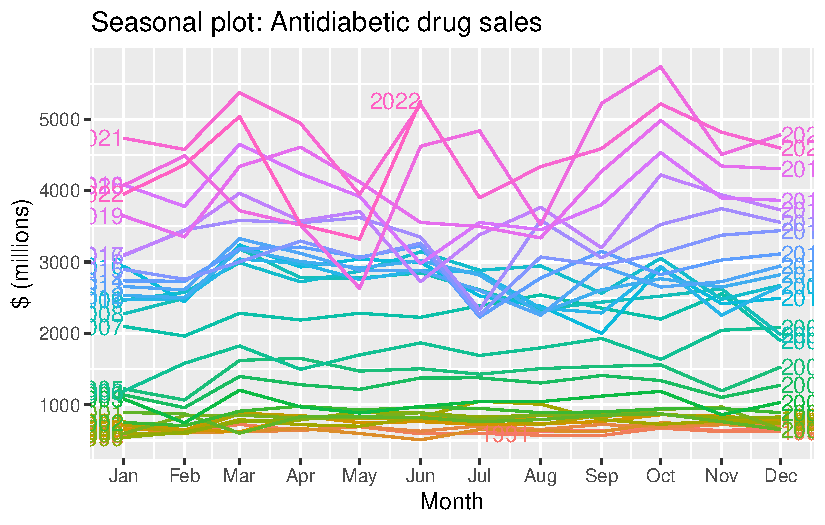
\includegraphics[width=17.1875in,height=\textheight]{cement_files/figure-pdf/unnamed-chunk-13-1.pdf}

}

\end{figure}

\hypertarget{monthly-analysis}{%
\subsection{Monthly Analysis}\label{monthly-analysis}}

\begin{Shaded}
\begin{Highlighting}[]
\NormalTok{cement }\SpecialCharTok{\%\textgreater{}\%}
  \FunctionTok{gg\_subseries}\NormalTok{(Output,}\AttributeTok{labels =} \StringTok{"both"}\NormalTok{)}\SpecialCharTok{+}
  \FunctionTok{labs}\NormalTok{(}\AttributeTok{y =} \StringTok{"$ (millions)"}\NormalTok{,}
       \AttributeTok{title =} \StringTok{"Seasonal plot: Antidiabetic drug sales"}\NormalTok{)}
\DocumentationTok{\#\# Warning: Ignoring unknown parameters: labels}
\end{Highlighting}
\end{Shaded}

\begin{figure}[H]

{\centering 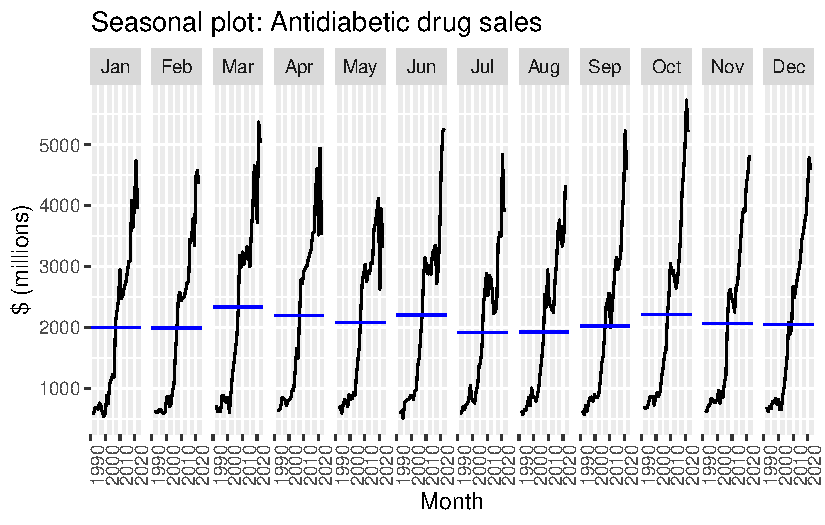
\includegraphics[width=17.1875in,height=\textheight]{cement_files/figure-pdf/unnamed-chunk-14-1.pdf}

}

\end{figure}

\hypertarget{lag-plots}{%
\subsection{Lag Plots}\label{lag-plots}}

\begin{Shaded}
\begin{Highlighting}[]

\NormalTok{cement }\SpecialCharTok{\%\textgreater{}\%}
  \FunctionTok{gg\_lag}\NormalTok{(Output, }\AttributeTok{geom =} \StringTok{"point"}\NormalTok{) }\SpecialCharTok{+}
  \FunctionTok{labs}\NormalTok{(}\AttributeTok{x =} \StringTok{"lag(Output, k)"}\NormalTok{)}
\end{Highlighting}
\end{Shaded}

\begin{figure}[H]

{\centering 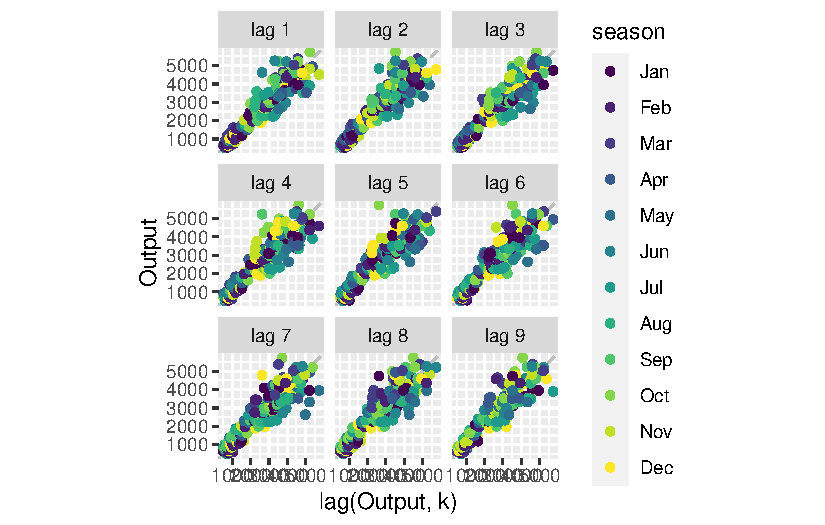
\includegraphics[width=17.1875in,height=\textheight]{cement_files/figure-pdf/unnamed-chunk-15-1.pdf}

}

\end{figure}

\hypertarget{shiny-interactive-view}{%
\subsection{Shiny Interactive View}\label{shiny-interactive-view}}

\begin{Shaded}
\begin{Highlighting}[]
\FunctionTok{library}\NormalTok{(seasonalview)}
\DocumentationTok{\#\# Loading required package: seasonal}
\DocumentationTok{\#\# }
\DocumentationTok{\#\# Attaching package: \textquotesingle{}seasonal\textquotesingle{}}
\DocumentationTok{\#\# The following object is masked from \textquotesingle{}package:tibble\textquotesingle{}:}
\DocumentationTok{\#\# }
\DocumentationTok{\#\#     view}
\DocumentationTok{\#\# }
\DocumentationTok{\#\# Attaching package: \textquotesingle{}seasonalview\textquotesingle{}}
\DocumentationTok{\#\# The following object is masked from \textquotesingle{}package:seasonal\textquotesingle{}:}
\DocumentationTok{\#\# }
\DocumentationTok{\#\#     view}
\DocumentationTok{\#\# The following object is masked from \textquotesingle{}package:tibble\textquotesingle{}:}
\DocumentationTok{\#\# }
\DocumentationTok{\#\#     view}
\FunctionTok{library}\NormalTok{(shiny)}
\DocumentationTok{\#\# }
\DocumentationTok{\#\# Attaching package: \textquotesingle{}shiny\textquotesingle{}}
\DocumentationTok{\#\# The following objects are masked from \textquotesingle{}package:DT\textquotesingle{}:}
\DocumentationTok{\#\# }
\DocumentationTok{\#\#     dataTableOutput, renderDataTable}
\CommentTok{\#cement\_prod\textless{}{-}ts(data = cement$Output,frequency = 12, start=c(1991,7))}
\CommentTok{\#view(seas(cement\_prod))}
\end{Highlighting}
\end{Shaded}

\begin{Shaded}
\begin{Highlighting}[]
\ExtensionTok{quarto}\NormalTok{ render cement.qmd }\AttributeTok{{-}{-}to}\NormalTok{ pdf}
\end{Highlighting}
\end{Shaded}




\end{document}
